%  LaTeX support: latex@mdpi.com
%  For support, please attach all files needed for compiling as well as the log file, and specify your operating system, LaTeX version, and LaTeX editor.

%=================================================================
% pandoc conditionals added to preserve backwards compatibility with previous versions of rticles
\documentclass[water,article,submit,oneauthor]{Definitions/mdpi}

% If you would like to post an early version of this manuscript as a preprint, you may use preprint as the journal and change 'submit' to 'accept'. The document class line would be, e.g., \documentclass[preprints,article,accept,moreauthors,pdftex]{mdpi}. This is especially recommended for submission to arXiv, where line numbers should be removed before posting. For preprints.org, the editorial staff will make this change immediately prior to posting.

%% Some pieces required from the pandoc template
\setlist[itemize]{leftmargin=*,labelsep=5.8mm}
\setlist[enumerate]{leftmargin=*,labelsep=4.9mm}


%--------------------
% Class Options:
%--------------------
%----------
% journal
%----------
% Choose between the following MDPI journals:
% acoustics, actuators, addictions, admsci, adolescents, aerobiology, aerospace, agriculture, agriengineering, agrochemicals, agronomy, ai, air, algorithms, allergies, alloys, analytica, analytics, anatomia, animals, antibiotics, antibodies, antioxidants, applbiosci, appliedchem, appliedmath, applmech, applmicrobiol, applnano, applsci, aquacj, architecture, arm, arthropoda, arts, asc, asi, astronomy, atmosphere, atoms, audiolres, automation, axioms, bacteria, batteries, bdcc, behavsci, beverages, biochem, bioengineering, biologics, biology, biomass, biomechanics, biomed, biomedicines, biomedinformatics, biomimetics, biomolecules, biophysica, biosensors, biotech, birds, bloods, blsf, brainsci, breath, buildings, businesses, cancers, carbon, cardiogenetics, catalysts, cells, ceramics, challenges, chemengineering, chemistry, chemosensors, chemproc, children, chips, cimb, civileng, cleantechnol, climate, clinpract, clockssleep, cmd, coasts, coatings, colloids, colorants, commodities, compounds, computation, computers, condensedmatter, conservation, constrmater, cosmetics, covid, crops, cryptography, crystals, csmf, ctn, curroncol, cyber, dairy, data, ddc, dentistry, dermato, dermatopathology, designs, devices, diabetology, diagnostics, dietetics, digital, disabilities, diseases, diversity, dna, drones, dynamics, earth, ebj, ecologies, econometrics, economies, education, ejihpe, electricity, electrochem, electronicmat, electronics, encyclopedia, endocrines, energies, eng, engproc, entomology, entropy, environments, environsciproc, epidemiologia, epigenomes, est, fermentation, fibers, fintech, fire, fishes, fluids, foods, forecasting, forensicsci, forests, foundations, fractalfract, fuels, future, futureinternet, futurepharmacol, futurephys, futuretransp, galaxies, games, gases, gastroent, gastrointestdisord, gels, genealogy, genes, geographies, geohazards, geomatics, geosciences, geotechnics, geriatrics, grasses, gucdd, hazardousmatters, healthcare, hearts, hemato, hematolrep, heritage, higheredu, highthroughput, histories, horticulturae, hospitals, humanities, humans, hydrobiology, hydrogen, hydrology, hygiene, idr, ijerph, ijfs, ijgi, ijms, ijns, ijpb, ijtm, ijtpp, ime, immuno, informatics, information, infrastructures, inorganics, insects, instruments, inventions, iot, j, jal, jcdd, jcm, jcp, jcs, jcto, jdb, jeta, jfb, jfmk, jimaging, jintelligence, jlpea, jmmp, jmp, jmse, jne, jnt, jof, joitmc, jor, journalmedia, jox, jpm, jrfm, jsan, jtaer, jvd, jzbg, kidneydial, kinasesphosphatases, knowledge, land, languages, laws, life, liquids, literature, livers, logics, logistics, lubricants, lymphatics, machines, macromol, magnetism, magnetochemistry, make, marinedrugs, materials, materproc, mathematics, mca, measurements, medicina, medicines, medsci, membranes, merits, metabolites, metals, meteorology, methane, metrology, micro, microarrays, microbiolres, micromachines, microorganisms, microplastics, minerals, mining, modelling, molbank, molecules, mps, msf, mti, muscles, nanoenergyadv, nanomanufacturing,\gdef\@continuouspages{yes}} nanomaterials, ncrna, ndt, network, neuroglia, neurolint, neurosci, nitrogen, notspecified, %%nri, nursrep, nutraceuticals, nutrients, obesities, oceans, ohbm, onco, %oncopathology, optics, oral, organics, organoids, osteology, oxygen, parasites, parasitologia, particles, pathogens, pathophysiology, pediatrrep, pharmaceuticals, pharmaceutics, pharmacoepidemiology,\gdef\@ISSN{2813-0618}\gdef\@continuous pharmacy, philosophies, photochem, photonics, phycology, physchem, physics, physiologia, plants, plasma, platforms, pollutants, polymers, polysaccharides, poultry, powders, preprints, proceedings, processes, prosthesis, proteomes, psf, psych, psychiatryint, psychoactives, publications, quantumrep, quaternary, qubs, radiation, reactions, receptors, recycling, regeneration, religions, remotesensing, reports, reprodmed, resources, rheumato, risks, robotics, ruminants, safety, sci, scipharm, sclerosis, seeds, sensors, separations, sexes, signals, sinusitis, skins, smartcities, sna, societies, socsci, software, soilsystems, solar, solids, spectroscj, sports, standards, stats, std, stresses, surfaces, surgeries, suschem, sustainability, symmetry, synbio, systems, targets, taxonomy, technologies, telecom, test, textiles, thalassrep, thermo, tomography, tourismhosp, toxics, toxins, transplantology, transportation, traumacare, traumas, tropicalmed, universe, urbansci, uro, vaccines, vehicles, venereology, vetsci, vibration, virtualworlds, viruses, vision, waste, water, wem, wevj, wind, women, world, youth, zoonoticdis
% For posting an early version of this manuscript as a preprint, you may use "preprints" as the journal. Changing "submit" to "accept" before posting will remove line numbers.

%---------
% article
%---------
% The default type of manuscript is "article", but can be replaced by:
% abstract, addendum, article, book, bookreview, briefreport, casereport, comment, commentary, communication, conferenceproceedings, correction, conferencereport, entry, expressionofconcern, extendedabstract, datadescriptor, editorial, essay, erratum, hypothesis, interestingimage, obituary, opinion, projectreport, reply, retraction, review, perspective, protocol, shortnote, studyprotocol, systematicreview, supfile, technicalnote, viewpoint, guidelines, registeredreport, tutorial
% supfile = supplementary materials

%----------
% submit
%----------
% The class option "submit" will be changed to "accept" by the Editorial Office when the paper is accepted. This will only make changes to the frontpage (e.g., the logo of the journal will get visible), the headings, and the copyright information. Also, line numbering will be removed. Journal info and pagination for accepted papers will also be assigned by the Editorial Office.

%------------------
% moreauthors
%------------------
% If there is only one author the class option oneauthor should be used. Otherwise use the class option moreauthors.

%---------
% pdftex
%---------
% The option pdftex is for use with pdfLaTeX. Remove "pdftex" for (1) compiling with LaTeX & dvi2pdf (if eps figures are used) or for (2) compiling with XeLaTeX.

%=================================================================
% MDPI internal commands - do not modify
\firstpage{1}
\makeatletter
\setcounter{page}{\@firstpage}
\makeatother
\pubvolume{1}
\issuenum{1}
\articlenumber{0}
\pubyear{2023}
\copyrightyear{2023}
%\externaleditor{Academic Editor: Firstname Lastname}
\datereceived{ }
\daterevised{ } % Comment out if no revised date
\dateaccepted{ }
\datepublished{ }
%\datecorrected{} % For corrected papers: "Corrected: XXX" date in the original paper.
%\dateretracted{} % For corrected papers: "Retracted: XXX" date in the original paper.
\hreflink{https://doi.org/} % If needed use \linebreak
%\doinum{}
%\pdfoutput=1 % Uncommented for upload to arXiv.org

%=================================================================
% Add packages and commands here. The following packages are loaded in our class file: fontenc, inputenc, calc, indentfirst, fancyhdr, graphicx, epstopdf, lastpage, ifthen, float, amsmath, amssymb, lineno, setspace, enumitem, mathpazo, booktabs, titlesec, etoolbox, tabto, xcolor, colortbl, soul, multirow, microtype, tikz, totcount, changepage, attrib, upgreek, array, tabularx, pbox, ragged2e, tocloft, marginnote, marginfix, enotez, amsthm, natbib, hyperref, cleveref, scrextend, url, geometry, newfloat, caption, draftwatermark, seqsplit
% cleveref: load \crefname definitions after \begin{document}

%=================================================================
% Please use the following mathematics environments: Theorem, Lemma, Corollary, Proposition, Characterization, Property, Problem, Example, ExamplesandDefinitions, Hypothesis, Remark, Definition, Notation, Assumption
%% For proofs, please use the proof environment (the amsthm package is loaded by the MDPI class).

%=================================================================
% Full title of the paper (Capitalized)
\Title{Assessing linkages between watershed nutrient loading and estuary
water quality in Lavaca Bay, Texas}

% MDPI internal command: Title for citation in the left column
\TitleCitation{Assessing linkages between watershed nutrient loading and
estuary water quality in Lavaca Bay, Texas}

% Author Orchid ID: enter ID or remove command
%\newcommand{\orcidauthorA}{0000-0000-0000-000X} % Add \orcidA{} behind the author's name
%\newcommand{\orcidauthorB}{0000-0000-0000-000X} % Add \orcidB{} behind the author's name


% Authors, for the paper (add full first names)
\Author{Michael
Schramm$^{1}$\href{https://orcid.org/0000-0003-1876-6592}
{\orcidicon}}


%\longauthorlist{yes}


% MDPI internal command: Authors, for metadata in PDF
\AuthorNames{Michael Schramm}

% MDPI internal command: Authors, for citation in the left column
%\AuthorCitation{Lastname, F.; Lastname, F.; Lastname, F.}
% If this is a Chicago style journal: Lastname, Firstname, Firstname Lastname, and Firstname Lastname.
\AuthorCitation{Schramm, M.}

% Affiliations / Addresses (Add [1] after \address if there is only one affiliation.)
\address{%
$^{1}$ \quad Texas A\&M AgriLife Research - Texas Water Resources
Institute 1001 Holleman Dr.~E. College Station, TX
77840-2118; \href{mailto:michael.schramm@ag.tamu.edu}{\nolinkurl{michael.schramm@ag.tamu.edu}}\\
}

% Contact information of the corresponding author
\corres{Correspondence: \href{mailto:michael.schramm@ag.tamu.edu}{\nolinkurl{michael.schramm@ag.tamu.edu}}}

% Current address and/or shared authorship








% The commands \thirdnote{} till \eighthnote{} are available for further notes

% Simple summary

%\conference{} % An extended version of a conference paper

% Abstract (Do not insert blank lines, i.e. \\)
\abstract{A single paragraph of about 200 words maximum. For research
articles, abstracts should give a pertinent overview of the work. We
strongly encourage authors to use the following style of structured
abstracts, but without headings: 1) Background: Place the question
addressed in a broad context and highlight the purpose of the study; 2)
Methods: Describe briefly the main methods or treatments applied; 3)
Results: Summarize the article's main findings; and 4) Conclusion:
Indicate the main conclusions or interpretations. The abstract should be
an objective representation of the article, it must not contain results
which are not presented and substantiated in the main text and should
not exaggerate the main conclusions.}


% Keywords
\keyword{estuary; nutrient loading; water quality; Texas}

% The fields PACS, MSC, and JEL may be left empty or commented out if not applicable
%\PACS{J0101}
%\MSC{}
%\JEL{}

%%%%%%%%%%%%%%%%%%%%%%%%%%%%%%%%%%%%%%%%%%
% Only for the journal Diversity
%\LSID{\url{http://}}

%%%%%%%%%%%%%%%%%%%%%%%%%%%%%%%%%%%%%%%%%%
% Only for the journal Applied Sciences
%\featuredapplication{Authors are encouraged to provide a concise description of the specific application or a potential application of the work. This section is not mandatory.}
%%%%%%%%%%%%%%%%%%%%%%%%%%%%%%%%%%%%%%%%%%

%%%%%%%%%%%%%%%%%%%%%%%%%%%%%%%%%%%%%%%%%%
% Only for the journal Data
%\dataset{DOI number or link to the deposited data set if the data set is published separately. If the data set shall be published as a supplement to this paper, this field will be filled by the journal editors. In this case, please submit the data set as a supplement.}
%\datasetlicense{License under which the data set is made available (CC0, CC-BY, CC-BY-SA, CC-BY-NC, etc.)}

%%%%%%%%%%%%%%%%%%%%%%%%%%%%%%%%%%%%%%%%%%
% Only for the journal Toxins
%\keycontribution{The breakthroughs or highlights of the manuscript. Authors can write one or two sentences to describe the most important part of the paper.}

%%%%%%%%%%%%%%%%%%%%%%%%%%%%%%%%%%%%%%%%%%
% Only for the journal Encyclopedia
%\encyclopediadef{For entry manuscripts only: please provide a brief overview of the entry title instead of an abstract.}

%%%%%%%%%%%%%%%%%%%%%%%%%%%%%%%%%%%%%%%%%%
% Only for the journal Advances in Respiratory Medicine
%\addhighlights{yes}
%\renewcommand{\addhighlights}{%

%\noindent This is an obligatory section in “Advances in Respiratory Medicine”, whose goal is to increase the discoverability and readability of the article via search engines and other scholars. Highlights should not be a copy of the abstract, but a simple text allowing the reader to quickly and simplified find out what the article is about and what can be cited from it. Each of these parts should be devoted up to 2~bullet points.\vspace{3pt}\\
%\textbf{What are the main findings?}
% \begin{itemize}[labelsep=2.5mm,topsep=-3pt]
% \item First bullet.
% \item Second bullet.
% \end{itemize}\vspace{3pt}
%\textbf{What is the implication of the main finding?}
% \begin{itemize}[labelsep=2.5mm,topsep=-3pt]
% \item First bullet.
% \item Second bullet.
% \end{itemize}
%}

%%%%%%%%%%%%%%%%%%%%%%%%%%%%%%%%%%%%%%%%%%


% tightlist command for lists without linebreak
\providecommand{\tightlist}{%
  \setlength{\itemsep}{0pt}\setlength{\parskip}{0pt}}



\usepackage{booktabs}
\usepackage{longtable}
\usepackage{array}
\usepackage{multirow}
\usepackage{wrapfig}
\usepackage{float}
\usepackage{colortbl}
\usepackage{pdflscape}
\usepackage{tabu}
\usepackage{threeparttable}
\usepackage{threeparttablex}
\usepackage[normalem]{ulem}
\usepackage{makecell}
\usepackage{xcolor}
\usepackage{siunitx}

  \newcolumntype{d}{S[
    input-open-uncertainty=,
    input-close-uncertainty=,
    parse-numbers = false,
    table-align-text-pre=false,
    table-align-text-post=false
  ]}
  

\begin{document}



%%%%%%%%%%%%%%%%%%%%%%%%%%%%%%%%%%%%%%%%%%

\hypertarget{introduction}{%
\section{Introduction}\label{introduction}}

Like many coastal areas globally, coastal watersheds along the Texas
Gulf coast are facing pressures from increasing population, increases in
point source and non-point source pollution and alterations to
freshwater flows that alter water quality in downstream estuaries
\citep{bricker_effects_2008, kennicuttWaterQualityGulf2017, bugica_water_2020}.
Despite these increasing pressures, national scale assessments have
classified coastal estuaries in Texas as moderate or lower for
exhibiting eutrophic conditions \citep{bricker_effects_2008}. However, a
suite of recent studies indicate that estuary water quality dynamics in
both agriculturally dominated and urban watersheds within Texas are in
fact expressing conditions that are increasingly conducive to algal
blooms and eutrophication
\citep{wetzWaterQualityDynamics2016, wetz_exceptionally_2017, bugica_water_2020, chinPhytoplanktonBiomassCommunity2022}.
With identification of localized areas of estuary water quality concern
along the Texas coast \citep{bugica_water_2020}, localized studies are
being prioritized to better inform management actions.

This project provides an assessment of nutrient loading and water
quality responses in Lavaca Bay, Texas. Lavaca Bay is a secondary bay in
the larger Matagorda Bay system located roughly halfway between Houston,
Texas and Corpus Christi, Texas. Lavaca Bay has faced substantial
challenges associated with legacy contamination but general water
quality parameters such as dissolved oxygen (DO), nutrients, and
biological parameters have been well within state water quality
standards. However, long-term declines of benthic fauna abundance,
biomass, and diversity in Lavaca Bay that are linked to reductions in
freshwater inflows and changes in estuary salinity
\citep{beserespollackLongtermTrendsResponse2011, palmerImpactsDroughtsLow2015, montagnaAssessmentRelationshipFreshwater2020}
and are a concern to local stakeholders. \citet{bugica_water_2020}
identified monotonic increases in total phosphorus (TP), orthophosphate,
total Kjeldahl nitrogen (TKN), and chlorophyll-\emph{a} at sites within
Lavaca Bay. Although no long-term changes in DO concentrations were
identified, the trends in nutrient concentrations are concerning due to
the role of nitrogen as a limiting factor for primary production in many
Texas estuaries
\citep{gardnerNitrogenFixationDissimilatory2006, houTransformationFateNitrate2012, doradoUnderstandingInteractionsFreshwater2015, paudelRelationshipSuspendedSolids2019, wetz_exceptionally_2017}
and the ramifications that major changes in nitrogen loadings could have
for productivity and eutrophication in Lavaca Bay.

There are ongoing efforts between local, state, and federal agencies to
address water quality impairments in the freshwater portions of the
Lavaca Bay watershed
\citep{jainTechnicalSupportDocument2021, schramm_lavaca_2018, bertholdDirectMailingEducation2021}.
However, at a statewide scale, these approaches have shown limited
success and emphasize a need for improved efforts at assessing and
linking management actions with downstream water quality to better
identify and replicate effective management actions across the state
\citep{schrammTotalMaximumDaily2022}. The identification and
communication of changes and trends in water quality is complicated by
the fact that trends are often non-linear and confounded by
precipitation and runoff that hinder traditional analysis
\citep{wazniakLinkingWaterQuality2007, lloydMethodsDetectingChange2014}.
To provide actionable information for resource managers, water quality
conditions must be evaluated relative to changes in natural
environmental drivers to better understand and manage potential
anthropogenic effects.

Here something some we present methodology and results for estimating
nutrient loading- and assessing linkages in estuary water quality
parameters with watershed derived nutrient loads\ldots.

\hypertarget{materials-and-methods}{%
\section{Materials and Methods}\label{materials-and-methods}}

\hypertarget{study-area-and-data}{%
\subsection{Study Area and Data}\label{study-area-and-data}}

\begin{figure}
\begin{adjustwidth}{-\extralength}{0cm}
\centering
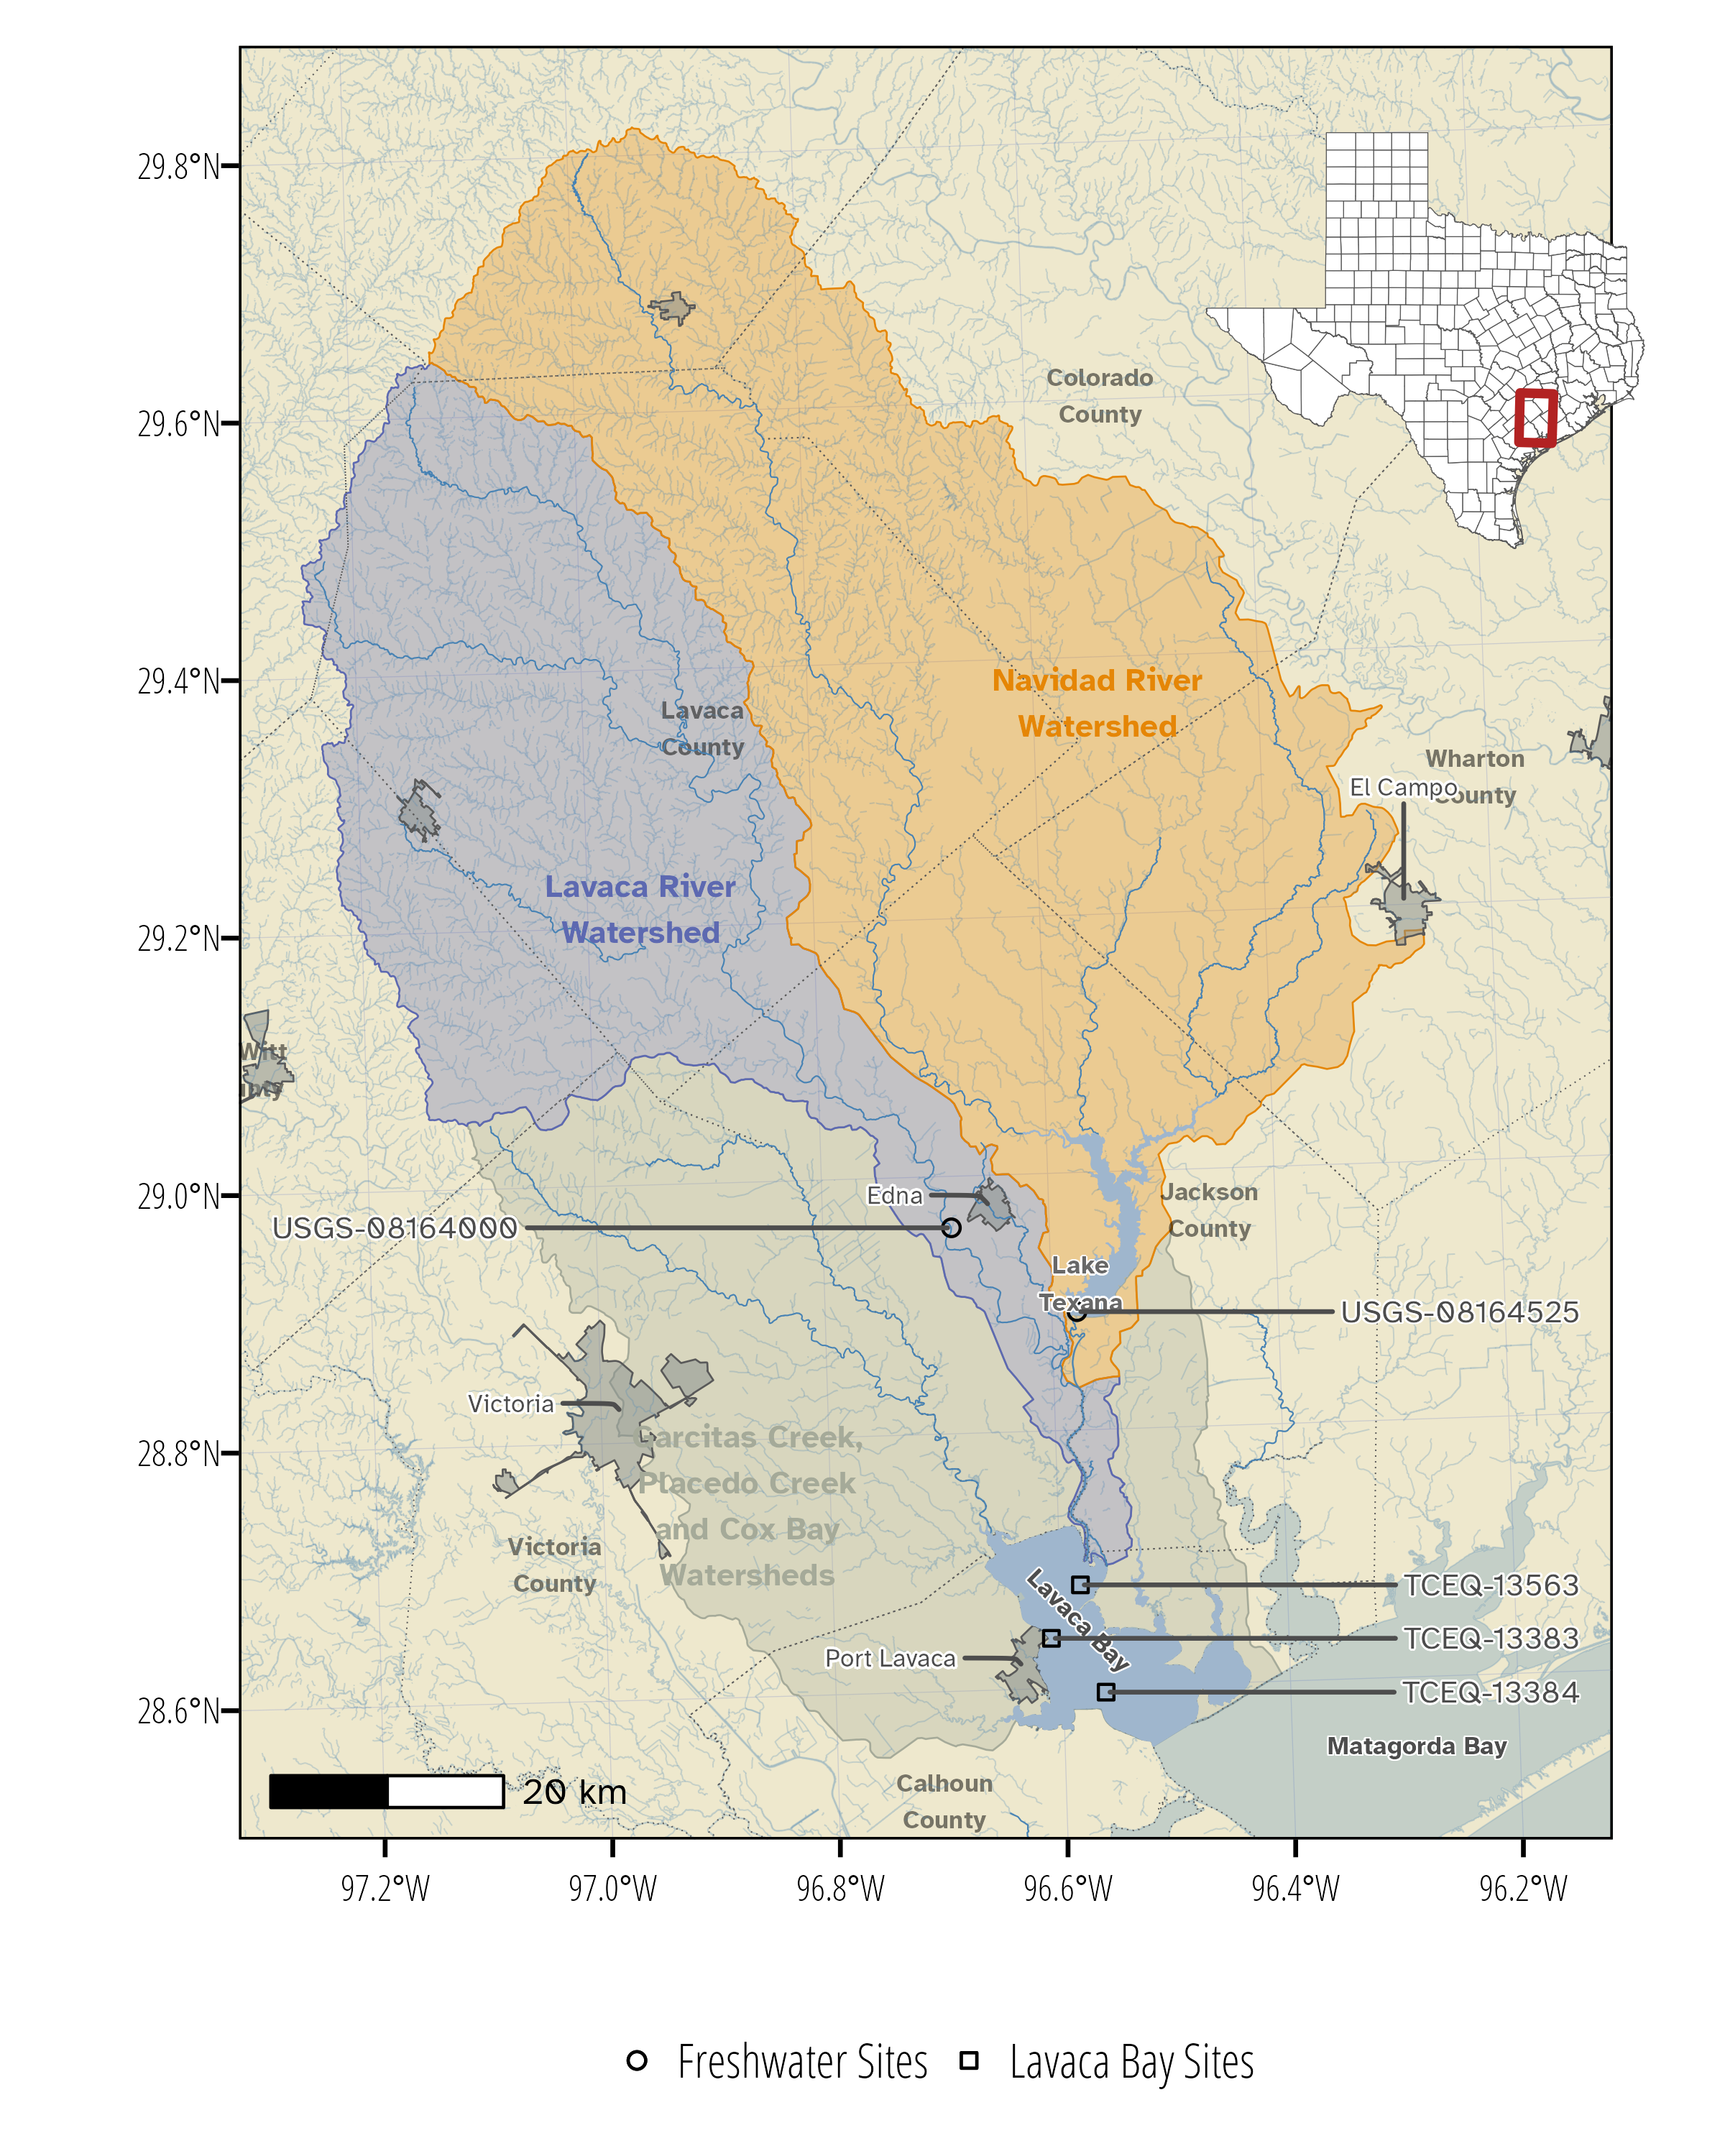
\includegraphics[width=15.5cm]{Schramm-Manuscript-2023_files/figure-latex/fig1-1.png}
\end{adjustwidth}
\caption{Map of the Lavaca Bay watershed, location of USGS gages where nutrient loads were calculated, and location of estuary water quality sampling sites.\label{fig1}}
\end{figure}

Lavaca Bay is a secondary bay in the Matagorda Bay system located on the
Texas Gulf coast, roughly halfway between the cities of Houston and
Corpus Christi (Figure \ref{fig:fig1}). Lavaca Bay is 190
km\textsuperscript{2} with the majority of freshwater inflow provided by
the Lavaca and Navidad River systems. The Garcitas-Arenosa, Placedo
Creek, and Cox Bay watersheds provide additional freshwater inflows. The
entire watershed land area for Lavaca Bay is 8,149
km\textsuperscript{2}. The Lavaca and Navidad River watersheds are a
combined 5,966 km\textsuperscript{2}, or approximately 73\% of the
entire Lavaca Bay watershed area. Discharge from the Navidad River is
regulated by Lake Texana which has been in operation since 1980. Lake
Texana provides 170,000 acre-feet of water storage and discharges into
the tidal section of the Navidad River which ultimately joins the tidal
section of the Lavaca River 15 km upstream of the confluence with the
Bay.

\textbf{Need to add a short description of land use}

Daily discharges for the Lavaca River (USGS-08164000, Figure
\ref{fig:fig1}) were obtained from the United States Geologic Survey
(USGS) National Water Information System using the \emph{dataRetrieval}
R package \citep{deciccoDataRetrievalPackagesDiscovering2022}. Gaged
daily discharges from the outlet of Lake Texana on the Navidad River
(USGS-0816425) were provided by the Texas Water Development Board (TWDB)
(April 21, 2022 email from R. Neupane, TWDB).

Water quality sample data for the two freshwater and three estuary
locations were obtained from the Texas Commission on Environmental
Quality (TCEQ) Surface Water Quality Monitoring Information System. Data
submitted through the system are required to be collected under Quality
Assurance Project Plans and lab method procedures outlined by the TCEQ's
procedures manual. The QAPP and procedures manuals ensure the consistent
collection and laboratory methods are applied between samples collected
by different entities and under different projects. All sites had
varying lengths of and availability of data. For freshwater locations,
TP from January 2000 through December 2020 and nitrate-nitrogen
(NO\textsubscript{3}) data from January 2005 through December 2020 were
downloaded (Table \ref{tab:fwsummary}). Less than 5-years of total
nitrogen and TKN concentration data were available at the freshwater
sites and deemed insufficient to develop load estimation models
(\textbf{CITE}). The three estuary sites included an upper Lavaca Bay
site near the outlet of the Lavaca River system (TCEQ-13563), a
mid-Lavaca Bay site (TCEQ-13383), and the lower Lavaca Bay site near the
mouth of the Bay (TCEQ-13384). For estuary locations, we obtained data
for TP, Nitrite+Nitrate (NO\emph{\textsubscript{x}}), TKN,
chlorophyll-\emph{a}, and DO concentrations from January 2005 through
December 2020 (Table \ref{tab:estuarysummary}).

\begin{table}[H]

\caption{\label{tab:fwsummary}Summary of gauged streamflow and freshwater water quality samples between January 1, 2000 and December 31, 2020.}
\centering
\begin{tabular}[t]{llrrr}
\toprule
Station ID &   & Mean & SD & N\\
\midrule
USGS-08164000 & TP (mg/L) & \num{0.21} & \num{0.09} & 80\\
 & NO\textsubscript{3} (mg/L) & \num{0.18} & \num{0.24} & 74\\
 & Mean Daily Streamflow (cfs) & \num{332.78} & \num{1667.47} & 7671\\
USGS-08164525 & TP (mg/L) & \num{0.20} & \num{0.08} & 81\\
 & NO\textsubscript{3} (mg/L) & \num{0.29} & \num{0.26} & 62\\
 & Mean Daily Streamflow (cfs) & \num{666.14} & \num{2957.79} & 7671\\
\bottomrule
\end{tabular}
\end{table}

\begin{table}[H]

\caption{\label{tab:estuarysummary}Summary of estuary water quality samples collected between January 1, 2005 and December 31, 2020.}
\centering
\begin{tabular}[t]{lllll}
\toprule
Station ID &   & Mean & SD & N\\
\midrule
 & TP (mg/L) & 0.11 & 0.05 & 47\\

 & NO\textsubscript{\emph{x}} (mg/L) & 0.07 & 0.15 & 51\\

 & TKN (mg/L) & 0.94 & 0.49 & 45\\

 & Chlorophyll-\emph{a} ($\mu$g/L) & 9.43 & 5.31 & 47\\

\multirow{-5}{*}{\raggedright\arraybackslash TCEQ-13383} & DO (mg/L) & 7.22 & 1.35 & 55\\
\cmidrule{1-5}
 & TP (mg/L) & 0.08 & 0.03 & 51\\

 & NO\textsubscript{\emph{x}} (mg/L) & 0.06 & 0.08 & 52\\

 & TKN (mg/L) & 0.76 & 0.40 & 48\\

 & Chlorophyll-\emph{a} ($\mu$g/L) & 8.22 & 6.44 & 46\\

\multirow{-5}{*}{\raggedright\arraybackslash TCEQ-13384} & DO (mg/L) & 7.51 & 1.32 & 54\\
\cmidrule{1-5}
 & TP (mg/L) & 0.13 & 0.06 & 50\\

 & NO\textsubscript{\emph{x}} (mg/L) & 0.09 & 0.13 & 53\\

 & TKN (mg/L) & 0.94 & 0.37 & 49\\

 & Chlorophyll-\emph{a} ($\mu$g/L) & 9.67 & 5.33 & 49\\

\multirow{-5}{*}{\raggedright\arraybackslash TCEQ-13563} & DO (mg/L) & 7.91 & 1.34 & 56\\
\bottomrule
\end{tabular}
\end{table}

\hypertarget{estimating-watershed-based-nutrient-loads}{%
\subsection{Estimating Watershed Based Nutrient
Loads}\label{estimating-watershed-based-nutrient-loads}}

Estimates of NO\textsubscript{3} and TP loads at the Lavaca River
(USGS-08164000) and the outlet of Lake Texana on the Navidad River
(USGS-08164250) were developed using Generalized Additive Models (GAMs)
relating nutrient concentration to river discharge, season, and time.
Separate models were fit at each station for each parameter and used to
predict nutrient concentrations for each day in the study period. GAMs
can be specified in a functionally similar manner to the commonly used
LOADEST \citep{cohn_validity_1992} or WRTDS \citep{hirsch_weighted_2010}
regression models and have been shown to produce reliable estimates of
nutrient and sediment loadings
\citep{wangLoadEstimationUncertainties2011, kroonRiverLoadsSuspended2012, kuhnert_quantifying_2012, robson_prediction_2015-1, hagemannEstimatingNutrientOrganic2016, mcdowell_implications_2021, biagi_novel_2022}.
GAMs are a semiparametric extension of generalized linear models where
the linear predictor is represented as the sum of multiple unknown
smooth functions and parametric linear predictors
\citep{wood_fast_2011}. Although the underlying parameter estimation
procedure of GAMs is substantially different than WRTDS, both the
functional form and results are demonstrated to be similar
\citep{beckNumericalQualitativeContrasts2017}. The use of GAMs over
other regression-based approaches was (1) the ability to easily explore
and incorporate different model terms, (2) the ability to incorporate
non-linear smooth function without explicit apriori knowledge of the
expect shape, and (3) the ability to specify a link function that
relates the expected value of the response to the linear predictors and
allows use to avoid data transformations as much as possible.

GAMs were fit using the \emph{mgcv} package in R which makes available
multiple types of smooth functions with automatic smoothness selection
\citep{wood_fast_2011}. The general form of the model relating
NO\textsubscript{3} and TP concentration to streamflow, season, and time
was:

\begin{equation}\label{eq:1}
\begin{aligned}
g(\mu) &= \alpha + f_1(ddate) + f_2(yday) + f_3(log1p(Q)) + f_4(ma) + f_5(fa)  \\
y &\sim \mathcal{N}(\mu,\,\sigma^{2}),
\end{aligned}
\end{equation}

where \(\mu\) is the conditional expected NO\textsubscript{3}-N or TP
concentration, \emph{g()} is the log-link, \(\alpha\) is the intercept,
\emph{f\textsubscript{n}()} are smoothing functions. \emph{y} is the
response variable (NO\textsubscript{3} or TP concentration) modeled as
normally distributed with mean \(\mu\) and standard deviation
\(\sigma\). \emph{ddate} is the date converted to decimal notation,
\emph{yday} is numeric day of year (1-366), and \emph{log1p(Q)} is the
natural log of mean daily streamflow plus 1.

Moving average (\emph{ma}) is an exponentially smoothed moving average
that attempts to incorporate the influence of prior streamflow events on
concentration at the current time period.
\citet{wangLoadEstimationUncertainties2011},
\citet{kuhnert_quantifying_2012} and \citet{zhang_improving_2017} refer
to this as averaged or smoothed discounted flow and demonstrated
improvements in nutrient loading models by including the term.
\citet{kuhnert_quantifying_2012} expresses \emph{ma} as:

\begin{equation}\label{eq:2}
ma(\delta) = d{\kappa_{i-1}}+(1-\delta)\hat{q}_{i-1}\quad\text{and}\quad \kappa_{i}=\sum_{m=1}^{i}\hat{Q}_m,
\end{equation}

where \(\delta\) is the discount factor (here, set equal to 0.95),
\(\kappa_i\) is the cumulative flow (\emph{Q}) up to the \emph{i}th day.

Flow anomaly (\emph{fa}) is a unitless term that represents how wet or
dry the current time period is from a previous time period
\citep{vecchia_trends_2009, zhang_improving_2017}. Long-term flow
anomaly (\emph{ltfa}) is the streamflow over the previous year relative
to the entire period and calculated as described by
\citet{zhang_improving_2017}:

\begin{equation}\label{eq:3}
ltfa(t) = \bar{x}_{1\,year}(t) - \bar{x}_{entire\,period} 
\end{equation}

and the short-term flow anomaly (\emph{stfa}) calculated as the current
day flow compared to the preceding 1-month streamflow:

\begin{equation}\label{eq:4}
stfa(t) = x_{current\,day}(t) - \bar{x}_{1\,month}(t) 
\end{equation}

where \emph{x} are the averages of log-transformed streamflow over the
antecedent period (\emph{1-year}, \emph{1-month}, etc.) for time
\emph{t}. We used \emph{ltfa} in NO\textasciitilde3 models and
\emph{stfa} in TP models based on results from
\citet{zhang_improving_2017} demonstrating major improvements in
NO\textsubscript{x} regression models that incorporated \emph{ltfa} and
moderate improvements in TP regression models that incorporated
\emph{stfa}.

The calculation of model terms for the Lake Texana site were slightly
modified because daily loads are not a function of natural stream flow
processes alone, but of dam releases and nutrient concentrations at the
discharge point of the lake. \emph{Q}, \emph{ma}, and \emph{fa} terms
were calculated based on total gaged inflow from the 4 major tributaries
to the lake. Thin-plate regression splines were used for \emph{ddate},
\emph{log1p(Q)}, \emph{fa}, and \emph{ma}. A cyclic cubic regression
spline was used for \emph{yday} to ensure the ends of the spline match
(day 1 and day 366 are expected to match). First order penalties were
applied to the smooths of flow-based variables which penalize departures
from a flat function to help constrain extrapolations for high flow
measurements.

Left-censored data were not uncommon in this dataset. Several methods
are available to account for censored data. We transformed left-censored
nutrient concentrations to one-half the detection limit. Although this
simple approach can introduce bias
\citep{hornungEstimationAverageConcentration1990}, we considered it
acceptable because high concentrations and loadings are associated with
high-flow events and low-flow/low-concentration events will account for
a small proportion of total loadings \citep{mcdowell_implications_2021}.

Daily loads were estimated as the predicted concentration multiplied by
the daily streamflow. For the Lake Texana site, model terms were
slightly modified because daily loads are a function of dam releases and
nutrient concentration, but concentration will be a function of lake
inflows and or other lake processes. \emph{Q}, \emph{ma}, and \emph{fa}
terms were calculated based on total gaged inflow from the 4 major
tributaries to the lake and laily loads at the dam were calculated from
the discrete daily concentration at the discharge point of the lake and
corresponding reported daily discharge from the dam. Flow-normalized
loads were estimated similar to WRTDS by setting flow-based covariates
on each day of the year equal to each of the historical values for that
day of the year over the study period \citep{hirsch_weighted_2010}. The
flow-normalized estimate was calculated as the mean of all the
predictions for each day considering all possible flow values. Standard
deviations and credible intervals were obtained by drawing samples from
the multivariate normal posterior distribution of the fitted GAM
\citep{woodConfidenceIntervalsGeneralized2006, marraCoveragePropertiesConfidence2012, mcdowell_implications_2021}.
Uncertainty in loads were reported as 90\% credible intervals developed
by drawing 1000 realizations of parameter estimates from the
multivariate normal posterior distribution of the model parameters. GAM
performance was evaluated using repeated 5-fold cross validation
\citep{burmanComparativeStudyOrdinary1989} and average Nash-Suttclifee
Efficiency (NSE), r\textsuperscript{2} and percent bias (PBIAS) metrics
across folds were calculated for each model.

\hypertarget{linking-estuary-water-quality-to-hydrology-and-nutrient-loads}{%
\subsection{Linking Estuary Water Quality to Hydrology and Nutrient
Loads}\label{linking-estuary-water-quality-to-hydrology-and-nutrient-loads}}

To test if changes in freshwater inflow and nutrient loading had
explanatory effect on changes in estuary water quality a series of GAM
models were fit at each site relating parameter concentration to
temporal trends, inflow, and nutrient loads
\citep{murphyNutrientImprovementsChesapeake2022}:

\begin{equation}\label{eq:5}
\begin{aligned}
g(\mu) &= \alpha + f_1(ddate) + f_2(yday) \\
y &\sim \Gamma(\mu,\lambda),
\end{aligned}
\end{equation}

\begin{equation}\label{eq:6}
\begin{aligned}
g(\mu) &= \alpha + f_1(ddate) + f_2(yday) + f_3(Q) \\
y &\sim \Gamma(\mu,\lambda),
\end{aligned}
\end{equation}

\begin{equation}\label{eq:7}
\begin{aligned}
g(\mu) &= \alpha + f_1(ddate) + f_2(yday) + f_3(Q) + f_4(Load) \\
y &\sim \Gamma(\mu,\lambda),
\end{aligned}
\end{equation}

where \(\mu\) is the conditional expected response (nutrient
concentration), \emph{g()} is the log link, and response variable was
modeled as Gamma distributed with mean \(\mu\) and scale \(\lambda\).
\emph{f\textsubscript{1}(ddate)} is decimal date smoothed with a
thin-plate regression spline, \emph{f\textsubscript{2}(yday)} is the
numeric day of year smoothed with a cyclic cubic regression spline,
\emph{f\textsubscript{3}(Q)} is mean daily inflow (the combined
measurements from Lavaca River and Lake Texana) and
\emph{f\textsubscript{4}(Load)} is the total NO\textsubscript{3} or TP
watershed load. The set of models specified for each water quality
response are in Table \ref{rab:estgammodels}.

\begin{table}[H]

\caption{\label{tab:estgammodels}Set of GAM models specified for each water quality parameter response.}
\centering
\begin{tabular}[t]{lll}
\toprule
\makecell[l]{Water Quality\\Response Parameter} & Model & Model Terms\\
\midrule
 & Temporal & s(ddate) + s(yday)\\

 & Flow & s(ddate) + s(yday) + s(Q)\\

\multirow{-3}{*}{\raggedright\arraybackslash TP} & Flow+Load & s(ddate) + s(yday) + s(Q) + s(TP Load)\\
\cmidrule{1-3}
 & Temporal & s(ddate) + s(yday)\\

 & Flow & s(ddate) + s(yday) + s(Q)\\

\multirow{-3}{*}{\raggedright\arraybackslash NO\textsubscript{\emph{x}}} & Flow+Load & s(ddate) + s(yday) + s(Q) + s(NO\textsubscript{3} Load)\\
\cmidrule{1-3}
 & Temporal & s(ddate) + s(yday)\\

 & Flow & s(ddate) + s(yday) + s(Q)\\

\multirow{-3}{*}{\raggedright\arraybackslash Chlorophyll-\emph{a}} & Flow+Load & s(ddate) + s(yday) + s(Q) + s(TP Load) + s(NO\textsubscript{3} Load)\\
\cmidrule{1-3}
 & Temporal & s(ddate) + s(yday)\\

 & Flow & s(ddate) + s(yday) + s(Q)\\

\multirow{-3}{*}{\raggedright\arraybackslash Dissolved Oxygen} & Flow+Load & s(ddate) + s(yday) + s(Q) + s(TP Load) + s(NO\textsubscript{3}  Load)\\
\cmidrule{1-3}
 & Temporal & s(ddate) + s(yday)\\

\multirow{-2}{*}{\raggedright\arraybackslash TKN} & Flow & s(ddate) + s(yday) + s(Q)\\
\bottomrule
\end{tabular}
\end{table}

Because streamflow and nutrient loads are tightly correlated, freshwater
inflow can mask signals from nutrient loads alone. Following the
methodology implemented by
\citet{murphyNutrientImprovementsChesapeake2022}, both streamflow and
nutrient loads were prepossessed to account for season and flow. Instead
of using raw freshwater inflow and nutrient loading values, these values
were replaced by seasonally adjusted inflow and flow-adjusted nutrient
loads by fitting a GAM relating season (day of year) to log transformed
daily freshwater inflow values:

\begin{equation}\label{eq:8}
g(\mu) = \alpha + f_1(yday),
\end{equation}

and a GAM relating log transformed NO\textsubscript{3} or TP loads to
log transformed daily inflow:

\begin{equation}\label{eq:9}
g(\mu) = \alpha + f_1(log(Q)),
\end{equation}

where the response variables were modeled as normally distributed with
an identity link function. Response residuals from the respective GAM
models were used as \emph{Q} and \emph{Load} in Equation \ref{eq:6} and
Equation \ref{eq:7}.

\hypertarget{results}{%
\section{Results}\label{results}}

\hypertarget{watershed-nutrient-loads}{%
\subsection{Watershed Nutrient Loads}\label{watershed-nutrient-loads}}

Based on criteria provided by \citet{moriasiHydrologicWaterQuality2015},
GAMs ranged from ``satisfactory'' to ``very good'' using median NSE,
r\textsuperscript{2} and PBIAS calculated using repeated 5-fold cross
validation on predicted and measured nutrient loads. NO\textsubscript{3}
GAM models had median NSE values of 0.34 and 0.48 at USGS-08164000 and
USGS-08164390 respectively. Median r\textsuperscript{2} values were 0.70
(USGS-08164000) and 0.87 (USGS-08164525) and PBIAS values were 2.00
(USGS-08164000) and 10.90 (USGS-08164525) for NO\textsubscript{3} loads.
Median NSE values were 0.80 (USGS-08164000) and 0.91 (USGS-08164525) for
TP loads. Median r\textsuperscript{2} values for TP loads were 0.93
(USGS-08164000) and 0.99 (USGS-08164525) and median PBIAS values were
-7.20 (USGS-08164000) and -3.30 (USGS-08164525). Density plots of
metrics show similar distribution of values between sites for the same
parameter, with the exception r\textsuperscript{2} values for
NO\textsubscript{3} loads where USGS-08164000 showed a much larger
variance in values compared to USGS-08164525 (Figure \ref{fig:fig2}).In
addition to higher average NSE and r\textsuperscript{2} values, GAMs had
smaller variance in metric values for TP compared to
NO\textsubscript{3}.

\begin{figure}\begin{adjustwidth}{-\extralength}{0cm}

{\centering 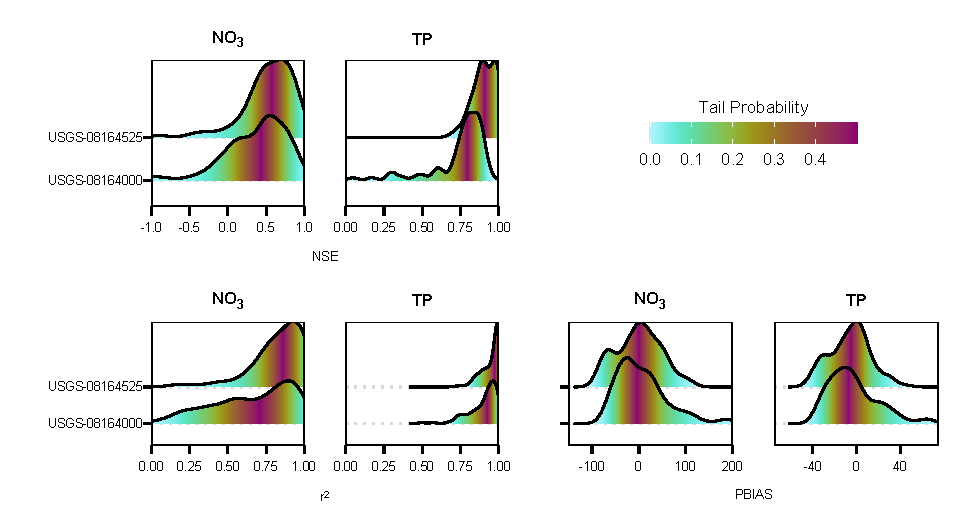
\includegraphics[width=1\linewidth]{Schramm-Manuscript-2023_files/figure-latex/fig2-1} 

}

\end{adjustwidth}\caption[Density plots of goodness-of-fit metrics (NSE, r\textsuperscript{2}, and PBIAS) from repeated 5-fold cross validation between predicted nutrient loads from GAM models and measured nutrient loads]{Density plots of goodness-of-fit metrics (NSE, r\textsuperscript{2}, and PBIAS) from repeated 5-fold cross validation between predicted nutrient loads from GAM models and measured nutrient loads. Color indicates the tail probability calcualted from the empirical cumulative distribution of the goodness-of-fit metrics.}\label{fig:fig2}
\end{figure}

Annual NO\textsubscript{3} and TP loads show considerable variation,
generally following patterns in discharge (Figure \ref{fig:fig3}, Figure
\ref{fig:fig4}). Flow-normalized TP loads at both sites and
flow-normalized loads at USGS-08164000 indicate watershed based loads
have not changed much over time when accounting for changes in
streamflow (Figure \ref{fig:fig3}). Flow-normalized loads at
USGS-08164000 show small variation over time with some decreases in
NO\textsubscript{3} loads since 2013. Aggregated across both sites, the
mean annual NO\textsubscript{3} load 2005 through 2020 was 205,405 kg
(126,867 kg - 341,569 kg, 90\% CI). Annual NO\textsubscript{3} loads
ranged from 12,574 kg in 2011 to 794,510 kg in 2007.

Total annual TP loads ranged from 7,839 kg in 2011 to 595,075 kg in
2007. Mean annual TP loading from 2005 through 2020 was 182,673 kg
(152,227 kg - 219,310 kg, 90\% CI). On average, USGS-08164525 accounted
for 68\% of NO\textsubscript{3} loads and 59\% of TP loads from 2005
through 2020. However, during periods of extreme drought the Lavaca
River (USGS-08164000) became the primary source of nutrient loading in
the watershed with the Navidad River only accounting for 15\% and 25\%
of NO\textsubscript{3} and TP loads in 2011 (Figure \ref{fig:fig4}).

\begin{figure}

{\centering 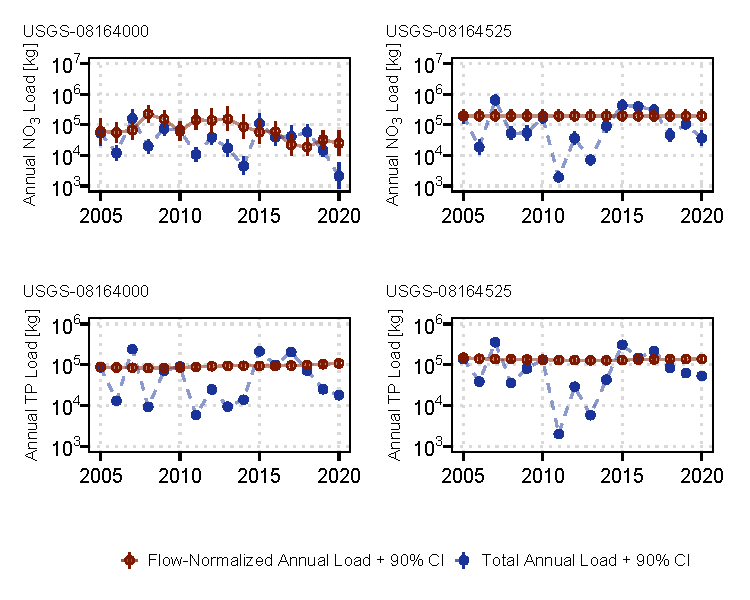
\includegraphics[width=1\linewidth]{Schramm-Manuscript-2023_files/figure-latex/fig3-1} 

}

\caption[Aggregated estimated annual and flow-normalized annual NO\textsubscript{3} and TP loads for USGS-08164000 and USGS-08164525]{Aggregated estimated annual and flow-normalized annual NO\textsubscript{3} and TP loads for USGS-08164000 and USGS-08164525.}\label{fig:fig3}
\end{figure}

\begin{figure}

{\centering 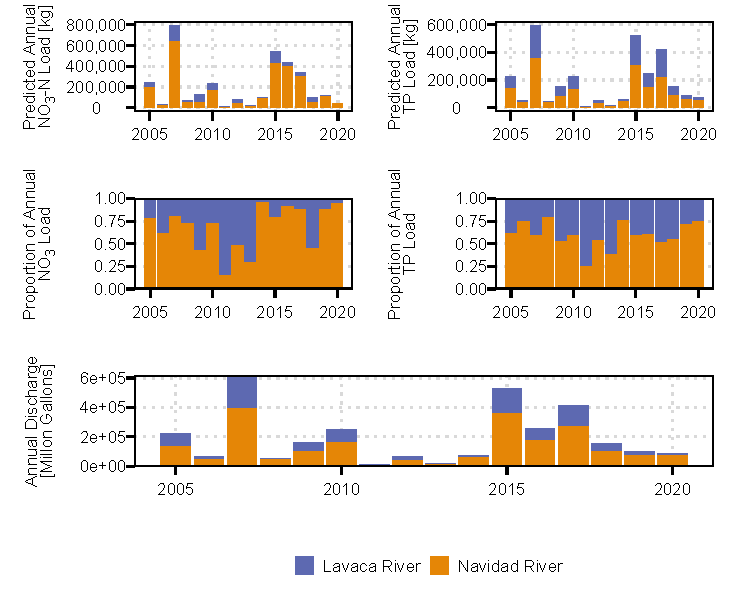
\includegraphics[width=1\linewidth]{Schramm-Manuscript-2023_files/figure-latex/fig4-1} 

}

\caption[Comparison of delivered annual loads at USGS-08164000 and USGS-08164525]{Comparison of delivered annual loads at USGS-08164000 and USGS-08164525.}\label{fig:fig4}
\end{figure}

\hypertarget{linkages-between-water-quality-and-watershed-flows-and-loads}{%
\subsection{Linkages Between Water Quality and Watershed Flows and
Loads}\label{linkages-between-water-quality-and-watershed-flows-and-loads}}

\begin{figure}\begin{adjustwidth}{-\extralength}{0cm}

{\centering 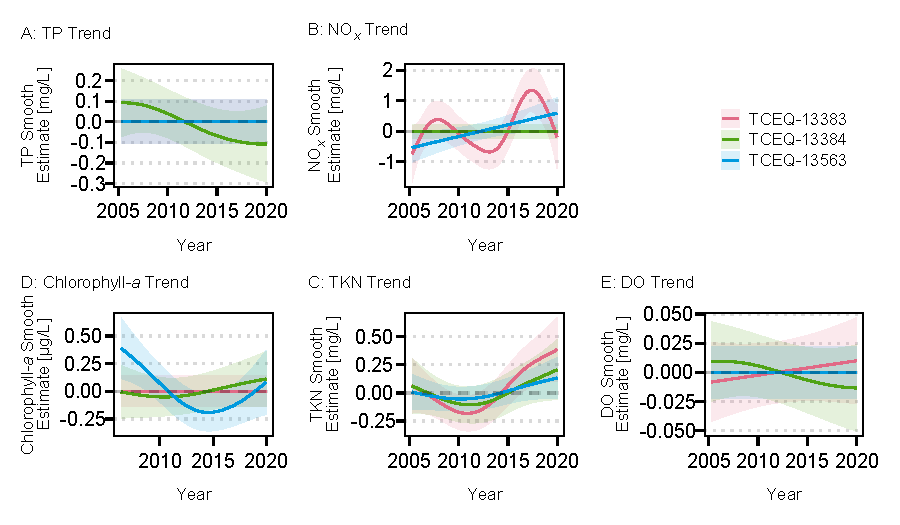
\includegraphics[width=1\linewidth]{Schramm-Manuscript-2023_files/figure-latex/fig5-1} 

}

\end{adjustwidth}\caption[Smoothed temporal trend component for water quality paramaters obtained from temporal estuary GAMs]{Smoothed temporal trend component for water quality paramaters obtained from temporal estuary GAMs.}\label{fig:fig5}
\end{figure}

GAMs did not identify significant changes in TP or DO concentrations at
any of the Lavaca Bay sites from 2005 through 2020 (Figure
\ref{fig:fig5}). The upper-bay site, TCEQ-13563, had a linear increase
in NO\textsubscript{x} concentration and and decrease in
chlorophyll-\emph{a} from 2005 through 2014. The mid-bay site,
TCEQ-13383, showed a periodic pattern in NO\textsubscript{x}
concentration that appeared similar to precipitation/inflow patterns, as
well as a post 2011 increase in TKN concentrations. No significant
long-term trends in concentrations were identified by GAMs for the
lower-bay TCEQ-13384 site.

Freshwater inflow provided additional explanation for changes in TP and
NO\textsubscript{\emph{x}} concentration at all of the Lavaca Bay sites
according to AIC\textsubscript{c} and model probability values (Table
\ref{tab:tab4}). TCEQ-13563, the site closest to the river outlet, was
the only site that had improvements in the explanations of DO and TKN
concentration with the inclusion of inflow. Both TCEQ-13563 and
TCEQ-13383, the mid-bay site, saw improvements in explanations for
variations in chlorophyll-\emph{a} with the inclusion of freshwater
inflow. The addition of nutrient loads (both TP and NO\textsubscript{3})
terms did not provide additional explanation for changes in
chlorophyll-\emph{a} or DO concentrations. Inclusion of TP loads
provided additional explanation of TP concentrations at the upper- and
mid-bay sites, TCEQ-13563 and TCEQ-13383. Inclusion of
NO\textsubscript{3} loads only provided marginal improvements in the
explanation of NO\textsubscript{\emph{X}} concentration at the lower-bay
TCEQ-13384 site.

\begin{table}[H]

\caption{\label{tab:tab4}Estuary GAM AIC\textsubscript{c} values and associated model probabilities (in parenthesis). Models with the highest probability for each site and water quality parameter combination are bolded and italicized for emphasis.}
\centering
\begin{tabular}[t]{ll>{}l>{}l>{}l}
\toprule
Parameter & Site & Temporal & Flow & Flow + Load\\
\midrule
 & TCEQ-13383 & -152.1 (0.03) & -156.1 (0.24) & \em{\textbf{-158.2 (0.72)}}\\

 & TCEQ-13384 & -194.4 (0.03) & \em{\textbf{-200.2 (0.49)}} & -200.2 (0.49)\\

\multirow{-3}{*}{\raggedright\arraybackslash TP} & TCEQ-13563 & -145.3 (0) & -156.6 (0.41) & \em{\textbf{-157.3 (0.59)}}\\
\cmidrule{1-5}
 & TCEQ-13383 & -218.9 (0) & \em{\textbf{-244.8 (0.5)}} & -244.8 (0.5)\\

 & TCEQ-13384 & -263.4 (0) & -311.7 (0.48) & \em{\textbf{-311.9 (0.52)}}\\

\multirow{-3}{*}{\raggedright\arraybackslash NO\textsubscript{\emph{x}}} & TCEQ-13563 & -175.1 (0) & \em{\textbf{-190.2 (0.5)}} & -190.2 (0.5)\\
\cmidrule{1-5}
 & TCEQ-13383 & 279.7 (0.18) & \em{\textbf{278.1 (0.41)}} & 278.1 (0.41)\\

 & TCEQ-13384 & \em{\textbf{268.2 (0.33)}} & 268.2 (0.33) & 268.2 (0.33)\\

\multirow{-3}{*}{\raggedright\arraybackslash Chlorophyll-\emph{a}} & TCEQ-13563 & 289.5 (0.08) & \em{\textbf{286.1 (0.46)}} & 286.1 (0.46)\\
\cmidrule{1-5}
 & TCEQ-13383 & \em{\textbf{42.2 (0.66)}} & 43.5 (0.34) & -\\

 & TCEQ-13384 & \em{\textbf{34.3 (0.57)}} & 34.8 (0.43) & -\\

\multirow{-3}{*}{\raggedright\arraybackslash TKN} & TCEQ-13563 & 31.1 (0.22) & \em{\textbf{28.7 (0.78)}} & -\\
\cmidrule{1-5}
 & TCEQ-13383 & \em{\textbf{146.4 (0.34)}} & 146.4 (0.34) & 146.5 (0.32)\\

 & TCEQ-13384 & \em{\textbf{135.9 (0.47)}} & 137 (0.27) & 137 (0.27)\\

\multirow{-3}{*}{\raggedright\arraybackslash DO} & TCEQ-13563 & 138.3 (0.25) & \em{\textbf{137.2 (0.43)}} & 137.8 (0.32)\\
\bottomrule
\end{tabular}
\end{table}

\begin{figure}\begin{adjustwidth}{-\extralength}{0cm}

{\centering 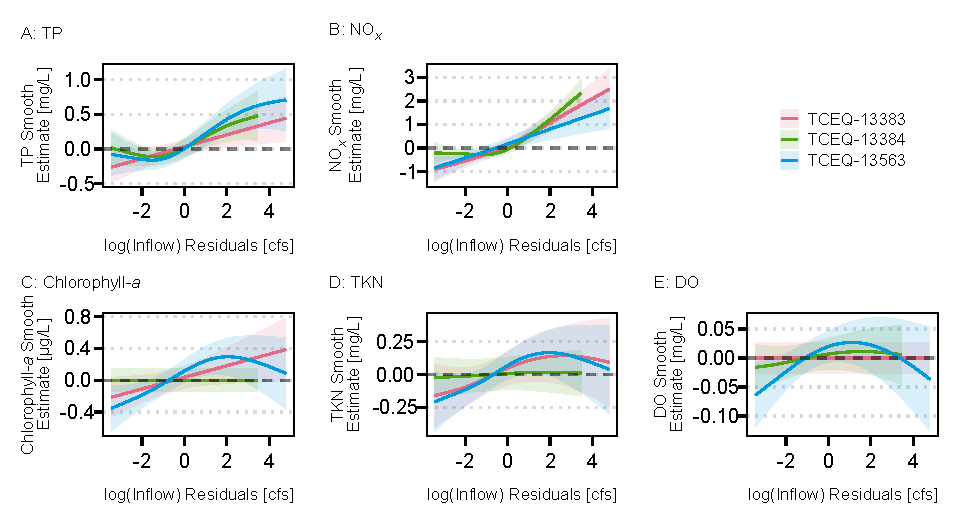
\includegraphics[width=1\linewidth]{Schramm-Manuscript-2023_files/figure-latex/fig6-1} 

}

\end{adjustwidth}\caption[Estimated effects of mean daily inflow residuals on mean TP, NO\textsubscript{\emph{x}}, chlorophyll-\emph{a}, TKN, and DO concentrations in Lavaca Bay obtained from flow estuary GAMs]{Estimated effects of mean daily inflow residuals on mean TP, NO\textsubscript{\emph{x}}, chlorophyll-\emph{a}, TKN, and DO concentrations in Lavaca Bay obtained from flow estuary GAMs.}\label{fig:fig6}
\end{figure}

GAMs show that increases in freshwater inflow result in nearly linear
increases in TP and NO\textsubscript{\emph{x}} at all three sites
(Figure \ref{fig:6}). At the upper-bay TCEQ-13563 site, GAMs showed
increases in freshwater inflow initially increased chlorophyll-\emph{a}
and DO concentration but concentrations leveled and potentially
decreased at higher flows. The mid-bay TCEQ-13383 site showed a nearly
linear increased in chlorophyll-\emph{a} concentration with increases in
freshwater inflow. Freshwater flow did not have significant effects on
chlorophyll-\emph{a}, TKN, or DO at the lower-bay TCEQ-13384 site.

Increases in TP loads resulted in nearly linear increases of TP
concentration at the upper- and mid-bay sites, TCEQ-13563 and TCEQ-13383
respectively (Figure \ref{fig:fig7}). The relative effect size appeared
to much smaller than the effect of freshwater inflow alone. Increases in
NO\textsubscript{3} loads only showed an effect at the lower-bay
TCEQ-13384 site. The effect was quite small compared to streamflow and
provided only small improvements to the model (Table \ref{tab:tab4}). As
noted above, nutrient loadings did not provide any explanation in
changes in the remaining assessed water quality parameters.

\begin{figure}

{\centering 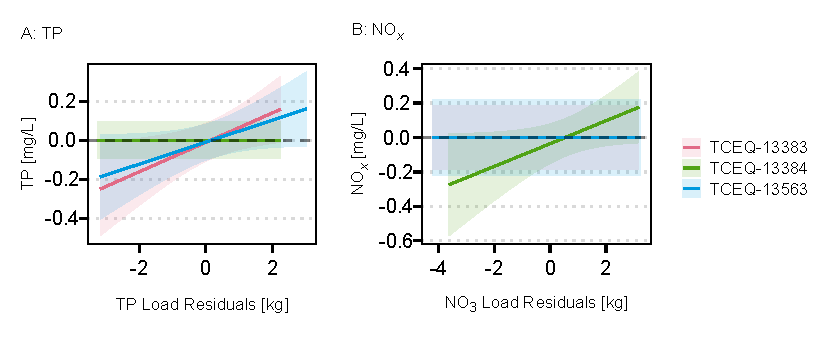
\includegraphics[width=1\linewidth]{Schramm-Manuscript-2023_files/figure-latex/fig7-1} 

}

\caption[Estimated effects of nutrient load residuals on TP and NO\textsubscript{\emph{x}} concentrations in Lavaca Bay obtained from flow+load estuary GAMs]{Estimated effects of nutrient load residuals on TP and NO\textsubscript{\emph{x}} concentrations in Lavaca Bay obtained from flow+load estuary GAMs.}\label{fig:fig7}
\end{figure}

\hypertarget{discussion}{%
\section{Discussion}\label{discussion}}

TP and NO\textsubscript{3} loadings from the Lavaca Bay watershed showed
high inter-annual variability tied with changes in discharge. There is
little evidence for changes in flow-normalized TP loads in either
rivers. There is some evidence of recent decreases in flow-normalized
NO\textsubscript{3} loads in the Lavaca River. Although there is no work
directly correlating water quality planning and implementation efforts
in the watershed to water quality outcomes, efforts to increase
agricultural producer participation in the watershed have been ongoing
since 2016
\citep{schramm_lavaca_2018, bertholdDirectMailingEducation2021}. The
decrease in flow-normalized NO\textsubscript{3} loads could be a
reflection of those collective efforts but further data collection and
research is required to support that statement.

Other studies have published estimates of TP loading estimates for the
Lavaca River (USGS-08164000) over various time periods (Table
\ref{tab:tpcomp}). Converted to average annual yield, the estimates of
TP loading in this study are within the ranges of previous studies
\citep{dunnTrendsNutrientInflows1996, rebich_sources_2011, omaniEstimationSedimentNutrient2014, wise_spatially_2019},
with the TP estimates in \citet{dunnTrendsNutrientInflows1996} being
notably lower. Given that none of the studies identify substantially
sized trends in TP, it is is possible that the period used in
\citet{dunnTrendsNutrientInflows1996} was drier on average than the
other studies. The SPARROW models used in \citet{rebich_sources_2011}
and \citet{wise_spatially_2019} utilize a version of LOADEST in the
underlying load estimation procedure, so a difference due to methodology
alone is unlikely.

\begin{table}[H]

\begin{threeparttable}
\caption{\label{tab:tpcomp}Mean estimates of annual TP yield in the Lavaca River watershed in published studies.}
\centering
\begin{tabular}[t]{lllll}
\toprule
Parameter & \makecell[c]{Reported Yield\\(kg$\cdot$km\textsuperscript{-2}$\cdot$year\textsuperscript{-1})} & Approach & Time Period & Reference\\
\midrule
TP & 35.2 (28.8, 43.3)\textsuperscript{*} & GAM & 2005-2020 & This work\\
TP & 45.2 & SPARROW & 2000-2014 & \citet{wise_spatially_2019}\\
TP & 42 & SWAT & 1977-2005 & \citet{omaniEstimationSedimentNutrient2014}\\
TP & 20.81-91.58\textsuperscript{\dag} & SPARROW & 1980-2002 & \citet{rebich_sources_2011}\\
TP & 28.9 & LOADEST & 1972-1993 & \citet{dunnTrendsNutrientInflows1996}\\
\bottomrule
\end{tabular}
\begin{tablenotes}
\small
\item [*] Values represent the mean of annual point estimates, lower and upper 95\% credible intervals.
\item [\dag] A single point estimate was not reported, these value represent the range depicted on the choropleth map provided in the report.
\end{tablenotes}
\end{threeparttable}
\end{table}

Cross-validation of the GAM loading models indicated that GAMs performed
well on average at predicting daily nutrient loading values. The
variance in scores was very high indicating subsets of values were
problematic at characterizing functional relationships between nutrients
and predictors. All of the water quality data for the two river sites in
the TCEQ database were ambient water quality data, collected to be
representative of typical conditions. This results in few data collected
at the highest portions of the flow duration curve under which the
majority of loadings take place. Supplementary flow-biased monitoring
targeting storm- or high-flow conditions is recommended here to improve
the precision of GAM predictions
\citep{horowitzEvaluationSedimentRating2003, snelderEstimationCatchmentNutrient2017}.

The non-linear temporal water quality trends identified using GAMs
differed slightly from the trends identified by
\citet{bugicaWaterQualityTrends2020}. This is not unexpected due to the
different time periods, different methodology, and generally small
slopes identified for most of the significant water quality parameters
in \citet{bugica_water_2020}. The trend in DO and cholorophyll-\emph{a}
concentrations are stable in comparison to other Texas estuaries that
might be facing larger demands for freshwater diversions, higher
population growth, and more intense agricultural production
\citep{wetzWaterQualityDynamics2016, bugica_water_2020}. The trend of
increasing NO\textsubscript{\emph{x}} concentration at the upper-bay
TCEQ-13563 site and recent increases in TKN concentration at the mid-bay
TCEQ-13383 site are concerning due to the nitrogen limitation identified
in many Texas estuaries
\citep{gardnerNitrogenFixationDissimilatory2006, houTransformationFateNitrate2012, doradoUnderstandingInteractionsFreshwater2015, paudelRelationshipSuspendedSolids2019, wetz_exceptionally_2017}
and the relatively low ambient concentrations observed in Lavaca Bay.

The strong positive effect of freshwater inflow on
NO\textsubscript{\emph{x}}, TKN, and TP are suggestive of nonpoint
watershed sources, consistent with watershed uses, and consistent with
other studies relating freshwater inflow with nutrient concentrations in
Lavaca Bay and other estuaries
\citep{russell_effect_2006, caffreyHighNutrientPulses2007, peierlsNonmonotonicResponsesPhytoplankton2012, palmerImpactsDroughtsLow2015, ciraPhytoplanktonDynamicsLowInflow2021}.
Inflow had a non-linear relationship with TKN at the two upstream sites,
with TKN increasing as freshwater inflow transitioned from low to
moderate levels. At higher freshwater inflows, the effect was
attenuated, possibly indicating a flushing effect at higher freshwater
inflow. No relationship between TKN and freshwater inflow were observed
at TCEQ-13384 located in the lower reach of Lavaca Bay. Tidal flushing
from Matagorda Bay might be responsible for decreasing TKN
concentrations and limiting the effects of freshwater inflow in lower
reaches of Lavaca Bay. \citet{russell_effect_2006} suggested the
processing of organic loads in the upper portions of Lavaca Bay reduces
the transport of nutrients into the lower reaches of the Bay.

Freshwater inflow also had a strong positive effect on
chlorophyll-\emph{a} at the upper- and mid-bay sites. The upper-bay
site, TCEQ-13563, showed decreases in chlorophyll-\emph{a} at the
highest freshwater inflow volumes. Freshwater flushing or increases in
turbidity are associated with decreases in chlorophyll-\emph{a} in other
estuaries
\citep{peierlsNonmonotonicResponsesPhytoplankton2012, cloernPhytoplanktonPrimaryProduction2014}.
No relationships between inorganic nitrogen or TP loadings with
chlorophyll-\emph{a} were observed. Due to the lack of TKN loading
information, no assessment between organic nitrogen loads and
chlorophyll-\emph{a} were possible.

Although other studies have identified complex relationships between
estuary nutrient concentrations, nutrient loading and
chlorophyll-\emph{a} concentrations in Texas estuaries
\citep{ornolfsdottirNutrientPulsingRegulator2004, doradoUnderstandingInteractionsFreshwater2015, ciraPhytoplanktonDynamicsLowInflow2021, tominackVariabilityPhytoplanktonBiomass2022},
this study specifically used flow-adjusted freshwater derived nutrient
loads to parse out contributions from changes in nutrient loadings while
accounting for variations in load due to flow. Loading GAMs indicated no
evidence of changes in flow-normalized TP loads in either river, and no
changes in flow-normalized NO\textsubscript{3} loads in the Navidad
River. The small changes in flow-normalized NO\textsubscript{3} loads in
the Lavaca River are probably masked under most conditions by discharge
from the Navidad River. Given the relatively little variation in
flow-normalized loads, it can be expected that they would contribute
little to the variance in downstream water quality.

GAMs did not identify responses in DO concentration to inflows or
nutrient loads. The seasonality term in the temporal GAM models
explained a substantial amount of DO variation at all of the sites.
Responses of estuary metabolic processes and resulting DO concentrations
can be quite complicated and often locally specific
\citep{caffreyFactorsControllingNet2004}. While the lack of total
nitrogen or TKN loading data hinders interpretation, the large seasonal
effect on DO suggests physical factors play an important role and should
be included in future models. Prior work suggests that there is some
evidence the Lavaca Bay may not be limited by nutrients alone, with high
turbidity or nutrient processing in upper portions of the Bay or
intertidal river limiting production \citep{russell_effect_2006}.

\hypertarget{conclusion}{%
\section{Conclusion}\label{conclusion}}

This section is not mandatory, but can be added to the manuscript if the
discussion is unusually long or complex.

%%%%%%%%%%%%%%%%%%%%%%%%%%%%%%%%%%%%%%%%%%

\vspace{6pt}

%%%%%%%%%%%%%%%%%%%%%%%%%%%%%%%%%%%%%%%%%%
%% optional

% Only for the journal Methods and Protocols:
% If you wish to submit a video article, please do so with any other supplementary material.
% \supplementary{The following supporting information can be downloaded at: \linksupplementary{s1}, Figure S1: title; Table S1: title; Video S1: title. A supporting video article is available at doi: link.}

%%%%%%%%%%%%%%%%%%%%%%%%%%%%%%%%%%%%%%%%%%

\funding{This paper was funded by financial assistance provided by the
Coastal Zone Management Act of 1972, as amended, administered by the
National Oceanic and Atmospheric Administration (NOAA), Office for
Coastal Management, pursuant to NOAA Award No.~NA21NOS4190136. The views
expressed herein are those of the author(s) and do not necessarily
reflect the views of NOAA, the U.S. Department of Commerce, or any of
their subagencies.}



\dataavailability{Data and code are openly available in Zenodo at
\url{https://doi.org/10.5281/zenodo.7330754}.}

\acknowledgments{Thank you to Mike Wetz (Harte Institute, Texas A\&M
Corpus Christi), Chad Kinsfather and Partick Brzozowski (Lavaca-Navidad
River Authority), Brian Koch (Texas State Soil and Water Conservation
Board), Bill Balboa (Matagorda Bay Foundation) and the Lavaca Bay
Foundation for supporting development of this project and providing
valuable feedback. Thank you to Ram Neupane (Texas Water Development
Board) for providing data.}

\conflictsofinterest{The author declares no conflict of interest. The
project sponsors had no role in the design of the study; in the
collection, analyses, or interpretation of data; in the writing of the
manuscript, or in the decision to publish the results.}

%%%%%%%%%%%%%%%%%%%%%%%%%%%%%%%%%%%%%%%%%%
%% Optional

%% Only for journal Encyclopedia
%\entrylink{The Link to this entry published on the encyclopedia platform.}


%%%%%%%%%%%%%%%%%%%%%%%%%%%%%%%%%%%%%%%%%%
%% Optional
%%%%%%%%%%%%%%%%%%%%%%%%%%%%%%%%%%%%%%%%%%
\begin{adjustwidth}{-\extralength}{0cm}

%\printendnotes[custom] % Un-comment to print a list of endnotes


\reftitle{References}

% Please provide either the correct journal abbreviation (e.g. according to the “List of Title Word Abbreviations” http://www.issn.org/services/online-services/access-to-the-ltwa/) or the full name of the journal.
% Citations and References in Supplementary files are permitted provided that they also appear in the reference list here.

%=====================================
% References, variant A: external bibliography
%=====================================
\externalbibliography{yes}
\bibliography{mybibfile.bib}

% If authors have biography, please use the format below
%\section*{Short Biography of Authors}
%\bio
%{\raisebox{-0.35cm}{\includegraphics[width=3.5cm,height=5.3cm,clip,keepaspectratio]{Definitions/author1.pdf}}}
%{\textbf{Firstname Lastname} Biography of first author}
%
%\bio
%{\raisebox{-0.35cm}{\includegraphics[width=3.5cm,height=5.3cm,clip,keepaspectratio]{Definitions/author2.jpg}}}
%{\textbf{Firstname Lastname} Biography of second author}

% For the MDPI journals use author-date citation, please follow the formatting guidelines on http://www.mdpi.com/authors/references
% To cite two works by the same author: \citeauthor{ref-journal-1a} (\citeyear{ref-journal-1a}, \citeyear{ref-journal-1b}). This produces: Whittaker (1967, 1975)
% To cite two works by the same author with specific pages: \citeauthor{ref-journal-3a} (\citeyear{ref-journal-3a}, p. 328; \citeyear{ref-journal-3b}, p.475). This produces: Wong (1999, p. 328; 2000, p. 475)

%%%%%%%%%%%%%%%%%%%%%%%%%%%%%%%%%%%%%%%%%%
%% for journal Sci
%\reviewreports{\\
%Reviewer 1 comments and authors’ response\\
%Reviewer 2 comments and authors’ response\\
%Reviewer 3 comments and authors’ response
%}
%%%%%%%%%%%%%%%%%%%%%%%%%%%%%%%%%%%%%%%%%%
\PublishersNote{}
\end{adjustwidth}


\end{document}
